%package list
\documentclass{article}
\usepackage[top=3cm, bottom=3cm, outer=3cm, inner=3cm]{geometry}
\usepackage{multicol}
\usepackage{graphicx}
\usepackage{url}
%\usepackage{cite}
\usepackage{hyperref}
\usepackage{array}
%\usepackage{multicol}
\newcolumntype{x}[1]{>{\centering\arraybackslash\hspace{0pt}}p{#1}}
\usepackage{natbib}
\usepackage{pdfpages}
\usepackage{multirow}
\usepackage[normalem]{ulem}
\useunder{\uline}{\ul}{}
\usepackage{svg}
\usepackage{xcolor}
\usepackage{listings}
\lstdefinestyle{ascii-tree}{
    literate={├}{|}1 {─}{--}1 {└}{+}1 
  }
\lstset{basicstyle=\ttfamily,
  showstringspaces=false,
  commentstyle=\color{red},
  keywordstyle=\color{blue}
}
%\usepackage{booktabs}
\usepackage{caption}
\usepackage{subcaption}
\usepackage{float}
\usepackage{array}

\newcolumntype{M}[1]{>{\centering\arraybackslash}m{#1}}
\newcolumntype{N}{@{}m{0pt}@{}}


%%%%%%%%%%%%%%%%%%%%%%%%%%%%%%%%%%%%%%%%%%%%%%%%%%%%%%%%%%%%%%%%%%%%%%%%%%%%
%%%%%%%%%%%%%%%%%%%%%%%%%%%%%%%%%%%%%%%%%%%%%%%%%%%%%%%%%%%%%%%%%%%%%%%%%%%%
\newcommand{\itemEmail}{schirinosne@unsa.edu.pe}
\newcommand{\itemStudent}{Sebastian Arley Chirinos Negrón}
\newcommand{\itemCourse}{Estructura de datos y Algoritmos}
\newcommand{\itemCourseCode}{1702124}
\newcommand{\itemSemester}{I}
\newcommand{\itemUniversity}{Universidad Nacional de San Agustín de Arequipa}
\newcommand{\itemFaculty}{Facultad de Ingeniería de Producción y Servicios}
\newcommand{\itemDepartment}{Departamento Académico de Ingeniería de Sistemas e Informática}
\newcommand{\itemSchool}{Escuela Profesional de Ingeniería de Sistemas}
\newcommand{\itemAcademic}{2023 - A}
\newcommand{\itemInput}{26 Junio 2023}
\newcommand{\itemOutput}{3 Julio 2023
}
\newcommand{\itemPracticeNumber}{06}
\newcommand{\itemTheme}{Arbol B+}
%%%%%%%%%%%%%%%%%%%%%%%%%%%%%%%%%%%%%%%%%%%%%%%%%%%%%%%%%%%%%%%%%%%%%%%%%%%%
%%%%%%%%%%%%%%%%%%%%%%%%%%%%%%%%%%%%%%%%%%%%%%%%%%%%%%%%%%%%%%%%%%%%%%%%%%%%

\usepackage[english,spanish]{babel}
\usepackage[utf8]{inputenc}
\AtBeginDocument{\selectlanguage{spanish}}
\renewcommand{\figurename}{Figura}
\renewcommand{\refname}{Referencias}
\renewcommand{\tablename}{Tabla} %esto no funciona cuando se usa babel
\AtBeginDocument{%
	\renewcommand\tablename{Tabla}
}

\usepackage{fancyhdr}
\pagestyle{fancy}
\fancyhf{}
\setlength{\headheight}{30pt}
\renewcommand{\headrulewidth}{1pt}
\renewcommand{\footrulewidth}{1pt}
\fancyhead[L]{\raisebox{-0.2\height}{
\includegraphics[width=3cm]{img/logo_episunsa.png}}}
\fancyhead[C]{\fontsize{7}{7}\selectfont	\itemUniversity \\ \itemFaculty \\ \itemDepartment \\ \itemSchool \\ \textbf{\itemCourse}}
\fancyhead[R]{\raisebox{-0.2\height}{
\includegraphics[width=1.2cm]{img/logo_abet}}}
\fancyfoot[L]{Sebastian Chirinos Negrón}
\fancyfoot[C]{\itemCourse}
\fancyfoot[R]{Página \thepage}

% para el codigo fuente
\usepackage{listings}
\usepackage{color, colortbl}
\definecolor{dkgreen}{rgb}{0,0.6,0}
\definecolor{gray}{rgb}{0.5,0.5,0.5}
\definecolor{mauve}{rgb}{0.58,0,0.82}
\definecolor{codebackground}{rgb}{72, 0.95, 0.92}
\definecolor{tablebackground}{rgb}{0.8, 0, 0}

\lstset{frame=tb,
	language=bash,
	aboveskip=3mm,
	belowskip=3mm,
	showstringspaces=false,
	columns=flexible,
	basicstyle={\small\ttfamily},
	numbers=none,
	numberstyle=\tiny\color{gray},
	keywordstyle=\color{blue},
	commentstyle=\color{dkgreen},
	stringstyle=\color{mauve},
	breaklines=true,
	breakatwhitespace=true,
	tabsize=3,
	backgroundcolor= \color{codebackground},
}

\begin{document}
	
	\vspace*{10px}
	
	\begin{center}	
		\fontsize{17}{17} \textbf{ Informe de Laboratorio \itemPracticeNumber}
	\end{center}
	\centerline{\textbf{\Large Tema: \itemTheme}}
	%\vspace*{0.5cm}	

	\begin{flushright}
		\begin{tabular}{|M{2.5cm}|N|}
			\hline 
			\rowcolor{tablebackground}
			\color{white} \textbf{Nota}  \\
			\hline 
			     \\[30pt]
			\hline 			
		\end{tabular}
	\end{flushright}	

	\begin{table}[H]
		\begin{tabular}{|x{4.7cm}|x{4.8cm}|x{4.8cm}|}
			\hline 
			\rowcolor{tablebackground}
			\color{white} \textbf{Estudiante} & \color{white}\textbf{Escuela}  & \color{white}\textbf{Asignatura}   \\
			\hline 
			{\itemStudent \par \itemEmail} & \itemSchool & {\itemCourse \par Semestre: \itemSemester \par Código: \itemCourseCode}     \\
			\hline 			
		\end{tabular}
	\end{table}		
	
	\begin{table}[H]
		\begin{tabular}{|x{4.7cm}|x{4.8cm}|x{4.8cm}|}
			\hline 
			\rowcolor{tablebackground}
			\color{white}\textbf{Laboratorio} & \color{white}\textbf{Tema}  & \color{white}\textbf{Duración}   \\
			\hline 
			\itemPracticeNumber & \itemTheme & 04 horas   \\
			\hline 
		\end{tabular}
	\end{table}
	
	\begin{table}[H]
		\begin{tabular}{|x{4.7cm}|x{4.8cm}|x{4.8cm}|}
			\hline 
			\rowcolor{tablebackground}
			\color{white}\textbf{Semestre académico} & \color{white}\textbf{Fecha de inicio}  & \color{white}\textbf{Fecha de entrega}   \\
			\hline 
			\itemAcademic & \itemInput &  \itemOutput  \\
			\hline 
		\end{tabular}
	\end{table}
	
	\section{Tarea}
	\begin{itemize}
		\item Introducción
En este informe, se presenta la implementación de B+.

	\end{itemize}	
		

	\section{URL de Repositorio Github}
	\begin{itemize}
		\item URL del Repositorio GitHub para clonar o recuperar.
		\item \url{https://github.com/BastleyNait/EDA-LAB-B-23A.git}
		\item URL para el laboratorio 04 en el Repositorio GitHub.
		\item \url{https://github.com/BastleyNait/EDA-LAB-B-23A/tree/main/lab03}
	\end{itemize}
	
	\section{Ejercicios designados}

	\subsection{Clase B+}
	\begin{itemize}
		\item Un B+ tree (árbol B+) es una estructura de datos de árbol equilibrado que se utiliza comúnmente en bases de datos y sistemas de almacenamiento para organizar y mantener grandes conjuntos de datos de manera eficiente. Es una extensión del árbol B, pero con algunas diferencias importantes que lo hacen especialmente adecuado para almacenar y recuperar datos en disco o en memoria secundaria.

\item Las principales características de un B+ tree son:

\item Nodos internos y hojas: Un B+ tree consta de nodos internos y hojas. Los nodos internos contienen claves y punteros a otros nodos internos o hojas. Las hojas contienen las claves y los datos almacenados.

\item Orden: El B+ tree tiene un orden que se refiere al número máximo de claves que puede contener un nodo. Por ejemplo, un B+ tree de orden 3 puede tener hasta 3 claves en cada nodo.

\item Claves ordenadas: Las claves en cada nodo están ordenadas de izquierda a derecha. Esto permite realizar búsquedas y operaciones de inserción y eliminación de manera eficiente utilizando búsqueda binaria.

\item Duplicados permitidos: Un B+ tree permite tener claves duplicadas, lo que significa que puede haber varios elementos con la misma clave en el árbol.

\item Propiedad de búsqueda: Todas las claves en un nodo interno actúan como "pivotes" que separan las claves de sus subárboles. Esto facilita la búsqueda y el enrutamiento a través del árbol.

\item Estructura de árbol equilibrado: Un B+ tree siempre mantiene una altura equilibrada, lo que garantiza tiempos de búsqueda y operaciones de inserción y eliminación en el orden de O(log n), donde "n" es el número de claves almacenadas.

\item Fusión y división: Cuando un nodo se llena o queda por debajo del mínimo permitido, se realiza la división o fusión de nodos para mantener el árbol equilibrado.

\item Debido a sus características, los B+ trees son ampliamente utilizados en sistemas de bases de datos y almacenamiento porque ofrecen una alta eficiencia para realizar búsquedas, inserciones y eliminaciones, y permiten realizar rápidamente operaciones de rango y ordenamiento en grandes conjuntos de datos.
	\end{itemize}

	\lstinputlisting[language=Java, caption={BPlustree.java},numbers=left,]{src/BPlustree.java}	

	\begin{itemize}
		\item Las principales características de un B+ tree son:

\item Nodos internos y hojas: Un B+ tree consta de nodos internos y hojas. Los nodos internos contienen claves y punteros a otros nodos internos o hojas. Las hojas contienen las claves y los datos almacenados.

\item Orden: El B+ tree tiene un orden que se refiere al número máximo de claves que puede contener un nodo. Por ejemplo, un B+ tree de orden 3 puede tener hasta 3 claves en cada nodo.

\item Claves ordenadas: Las claves en cada nodo están ordenadas de izquierda a derecha. Esto permite realizar búsquedas y operaciones de inserción y eliminación de manera eficiente utilizando búsqueda binaria.

\item Duplicados permitidos: Un B+ tree permite tener claves duplicadas, lo que significa que puede haber varios elementos con la misma clave en el árbol.

\item Propiedad de búsqueda: Todas las claves en un nodo interno actúan como "pivotes" que separan las claves de sus subárboles. Esto facilita la búsqueda y el enrutamiento a través del árbol.

\item Estructura de árbol equilibrado: Un B+ tree siempre mantiene una altura equilibrada, lo que garantiza tiempos de búsqueda y operaciones de inserción y eliminación en el orden de O(log n), donde "n" es el número de claves almacenadas.

\item Fusión y división: Cuando un nodo se llena o queda por debajo del mínimo permitido, se realiza la división o fusión de nodos para mantener el árbol equilibrado.

\item Debido a sus características, los B+ trees son ampliamente utilizados en sistemas de bases de datos y almacenamiento porque ofrecen una alta eficiencia para realizar búsquedas, inserciones y eliminaciones, y permiten realizar rápidamente operaciones de rango y ordenamiento en grandes conjuntos de datos.
	\end{itemize}

	%%%%%%%%%%%%%%%%%%%%%%%%%%%%%%%%%%%%%%%%%%%%%%%%%%%%%%%%%%%%%%%%%%%%%%%%%%%%%%%%%%%%%%%%%%%%%
	\subsection{Clase BPlusNode}
	\begin{itemize}	
		\item En resumen, esta clase Nodo representa un nodo en un árbol binario, utilizado en el contexto del BPlustree. Cada nodo contiene un dato, referencias a los nodos hijo izquierdo y derecho, y un campo para almacenar la altura del nodo. Proporciona métodos para acceder y modificar estos campos, así como métodos para obtener representaciones del nodo y realizar diferentes recorridos en profundidad en el árbol.
	\end{itemize}	
	
	\lstinputlisting[language=Java, caption={BPlusNode.java},numbers=left,]{src/BPlusNode.java}	

	\begin{itemize}
		\item Este código implementa la estructura de un árbol B+ en Java utilizando listas enlazadas para los nodos y punteros.

	\item Un árbol B+ es una variante de un árbol B que se utiliza comúnmente en bases de datos y sistemas de almacenamiento para organizar y buscar grandes conjuntos de datos de manera eficiente.

\item En esta implementación, la clase BPlusNode representa un nodo del árbol B+. Cada nodo contiene una lista de claves y una lista de punteros a otros nodos. Los nodos pueden ser nodos hoja (isLeaf = true) que almacenan datos o nodos internos (isLeaf = false) que se utilizan para organizar la estructura del árbol.

\end{itemize}
%%%%%%%%%%%%%%%%%%%%%%%%%%%%%%%%%%%%%%%%%%%%%%%%%%%%%%%%%%%%%%%%%%%%%%%%%%%%%%%%%%%%%%%%%%%%%%%%%%%%%%%%%%
%%%%%%%%%%%%%%%%%%%%%%%%%%%%%%%%%%%%%%%%%%%%%%%%%%%%%%%%%%%%%%%%%%%%%%%%%%%%%%%%%%%%%%%%%%%%%
\subsection{Clase Main}
\begin{itemize}	
	\item La clase main utiliza el árbol b+ para generar y manipular un árbol B+.
\end{itemize}	
\lstinputlisting[language=Java, caption={Main.java},numbers=left,]{src/Main.java}	
\begin{itemize}
	\item Este código es un programa principal en Java que utiliza la implementación de un árbol B+ (BPlusTree) para insertar claves y buscar valores en el árbol.

\item El programa comienza creando una instancia de BPlusTree llamada bpt. Luego, invoca el método insertarKeys() para insertar claves en el árbol bpt a través de la entrada del usuario. Después de insertar las claves, se llama al método printTree() para imprimir el contenido del árbol.

\item A continuación, el programa solicita al usuario que ingrese un valor para buscar en el árbol utilizando el método buscar(). El valor ingresado se pasa al método search() del árbol bpt, que realiza una búsqueda en el árbol y devuelve un valor booleano que indica si la clave se encuentra o no en el árbol. El resultado de la búsqueda se imprime en la consola.

\item En resumen, este programa permite al usuario insertar claves en un árbol B+ y luego buscar valores específicos en el árbol.
\end{itemize}

%%%%%%%%%%%%%%%%%%%%%%%%%%%%%%%%%%%%%%%%%%%%%%%%%%%%%%%%%%%%%%%%%%%%%%%%%%%%%%%%%%%%%%%%%%%%%%%%%%



%%%%%%%%%%%%%%%%%%%%%%%%%%%%%%%%%%%%%%%%%%%%%%%%%%%%%%%%%%%%%%%%%%%%%%%%%%%%%%%%%%


	\subsection{Commits del trabajo}
	\begin{itemize}	
		\item Acá estan algunos de los commits mas importantes en este trabajo:
	\end{itemize}	
	
	\begin{figure}[H]
		\centering
		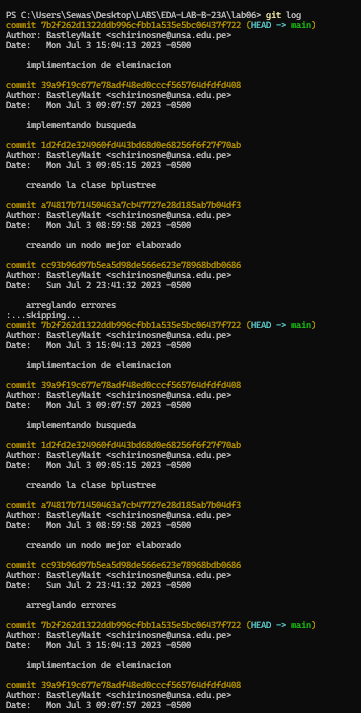
\includegraphics[width=0.7\textwidth,keepaspectratio]{img/Commits.png}
		%\includesvg{img/automata.svg}
		%\label{img:mot2}
		%\caption{Product backlog.}
	\end{figure}


%%%%%%%%%%%%%%%%%%%%%%%%%%%%%%%%%%%%%%%%%%%%%%%%%%%%%%%%%%%%%%%%%%%%%%%%%%%%%%%%%%
	
		
	\subsection{Estructura de laboratorio 06}
	\begin{itemize}	
		\item El contenido que se entrega en este laboratorio es el siguiente:
	\end{itemize}
	
\begin{lstlisting}[style=ascii-tree]
lab06/
|   .gitignore
|	BPlustree.java
|	BPlusNode.java
|	Main.java

\---latex
    |	EDA_lab06_schirinosne.pdf
    |   EDA_lab06_schirinosne.tex
    |
    +---img
    |       Commits.png
    |       logo_abet.png
    |       logo_episunsa.png
    |       logo_unsa.jpg
    |
    \---src
	|		BPlustree.java
	|		BPlusNode.java
	|		Main.java
\end{lstlisting}    


	\section{\textcolor{red}{Rúbricas}}
	
	\subsection{\textcolor{red}{Entregable Informe}}
	\begin{table}[H]
		\caption{Tipo de Informe}
		\setlength{\tabcolsep}{0.5em} % for the horizontal padding
		{\renewcommand{\arraystretch}{1.5}% for the vertical padding
		
		\begin{tabular}{|p{3cm}|p{12cm}|}
			\hline
			\multicolumn{2}{|c|}{\textbf{\textcolor{red}{Informe}}}  \\
			\hline 
			\textbf{\textcolor{red}{Latex}} & \textcolor{blue}{El informe está en formato PDF desde Latex,  con un formato limpio (buena presentación) y facil de leer.}   \\ 
			\hline 
			
			
		\end{tabular}
	}
	\end{table}
	\subsection{\textcolor{red}{Rúbrica para el contenido del Informe y demostración}}
	\begin{itemize}			
		\item El alumno debe marcar o dejar en blanco en celdas de la columna \textbf{Checklist} si cumplio con el ítem correspondiente.
		\item Si un alumno supera la fecha de entrega,  su calificación será sobre la nota mínima aprobada, siempre y cuando cumpla con todos lo items.
		\item El alumno debe autocalificarse en la columna \textbf{Estudiante} de acuerdo a la siguiente tabla:
	
		\begin{table}[ht]
			\caption{Niveles de desempeño}
			\begin{center}
			\begin{tabular}{ccccc}
    			\hline
    			 & \multicolumn{4}{c}{Nivel}\\
    			\cline{1-5}
    			\textbf{Puntos} & Insatisfactorio 25\%& En Proceso 50\% & Satisfactorio 75\% & Sobresaliente 100\%\\
    			\textbf{2.0}&0.5&1.0&1.5&2.0\\
    			\textbf{4.0}&1.0&2.0&3.0&4.0\\
    		\hline
			\end{tabular}
		\end{center}
	\end{table}	
	
	\end{itemize}
	
	\begin{table}[H]
		\caption{Rúbrica para contenido del Informe y demostración}
		\setlength{\tabcolsep}{0.5em} % for the horizontal padding
		{\renewcommand{\arraystretch}{1.5}% for the vertical padding
		%\begin{center}
		\begin{tabular}{|p{2.7cm}|p{7cm}|x{1.3cm}|p{1.2cm}|p{1.5cm}|p{1.1cm}|}
			\hline
    		\multicolumn{2}{|c|}{Contenido y demostración} & Puntos & Checklist & Estudiante & Profesor\\
			\hline
			\textbf{1. GitHub} & Hay enlace URL activo del directorio para el  laboratorio hacia su repositorio GitHub con código fuente terminado y fácil de revisar. &2 &X &2 & \\ 
			\hline
			\textbf{2. Commits} &  Hay capturas de pantalla de los commits más importantes con sus explicaciones detalladas. (El profesor puede preguntar para refrendar calificación). &4 & x&4 & \\ 
			\hline 
			\textbf{3. Código fuente} &  Hay porciones de código fuente importantes con numeración y explicaciones detalladas de sus funciones. &2 &X &2 & \\ 
			\hline 
			\textbf{4. Ejecución} & Se incluyen ejecuciones/pruebas del código fuente  explicadas gradualmente. &2 &X &2 & \\ 
			\hline			
			\textbf{5. Pregunta} & Se responde con completitud a la pregunta formulada en la tarea.  (El profesor puede preguntar para refrendar calificación).  &2 &X &2 & \\ 
			\hline	
			\textbf{6. Fechas} & Las fechas de modificación del código fuente estan dentro de los plazos de fecha de entrega establecidos. &2 &X &2 & \\ 
			\hline 
			\textbf{7. Ortografía} & El documento no muestra errores ortográficos. &2 &X &2 & \\ 
			\hline 
			\textbf{8. Madurez} & El Informe muestra de manera general una evolución de la madurez del código fuente,  explicaciones puntuales pero precisas y un acabado impecable.   (El profesor puede preguntar para refrendar calificación).  &4 &x &2 & \\ 
			\hline
			\multicolumn{2}{|c|}{\textbf{Total}} &20 & &18 & \\ 
			\hline
		\end{tabular}
		%\end{center}
		%\label{tab:multicol}
		}
	\end{table}
	
\clearpage		
\section{Referencias}
\begin{itemize}			
	\item \url{https://www.geeksforgeeks.org/introduction-to-avl-tree/}
	\item \url{https://www.geeksforgeeks.org/insertion-in-an-avl-tree/}
	\item \url{https://www.geeksforgeeks.org/deletion-in-an-avl-tree/}
	\item \url{https://docs.oracle.com/javase/tutorial/java/generics/types.html}
	\item \url{https://algorithmtutor.com/Data-Structures/Tree/AVL-Trees/}

\end{itemize}	

	
%\clearpage
%\bibliographystyle{apalike}
%\bibliographystyle{IEEEtranN}
%\bibliography{bibliography}
			
\end{document}